\item

$\text{grad} f = \vec \nabla f(x,y) = \tvect{\frac{\partial}{\partial x}}{\frac{\partial}{\partial y}} f(x,y) = \tvect{\cos(x)\sin(y)}{\sin(x)\cos(y)}$ Siehe unten für Abbildungen.

\begin{figure}[ht]
  \centering
  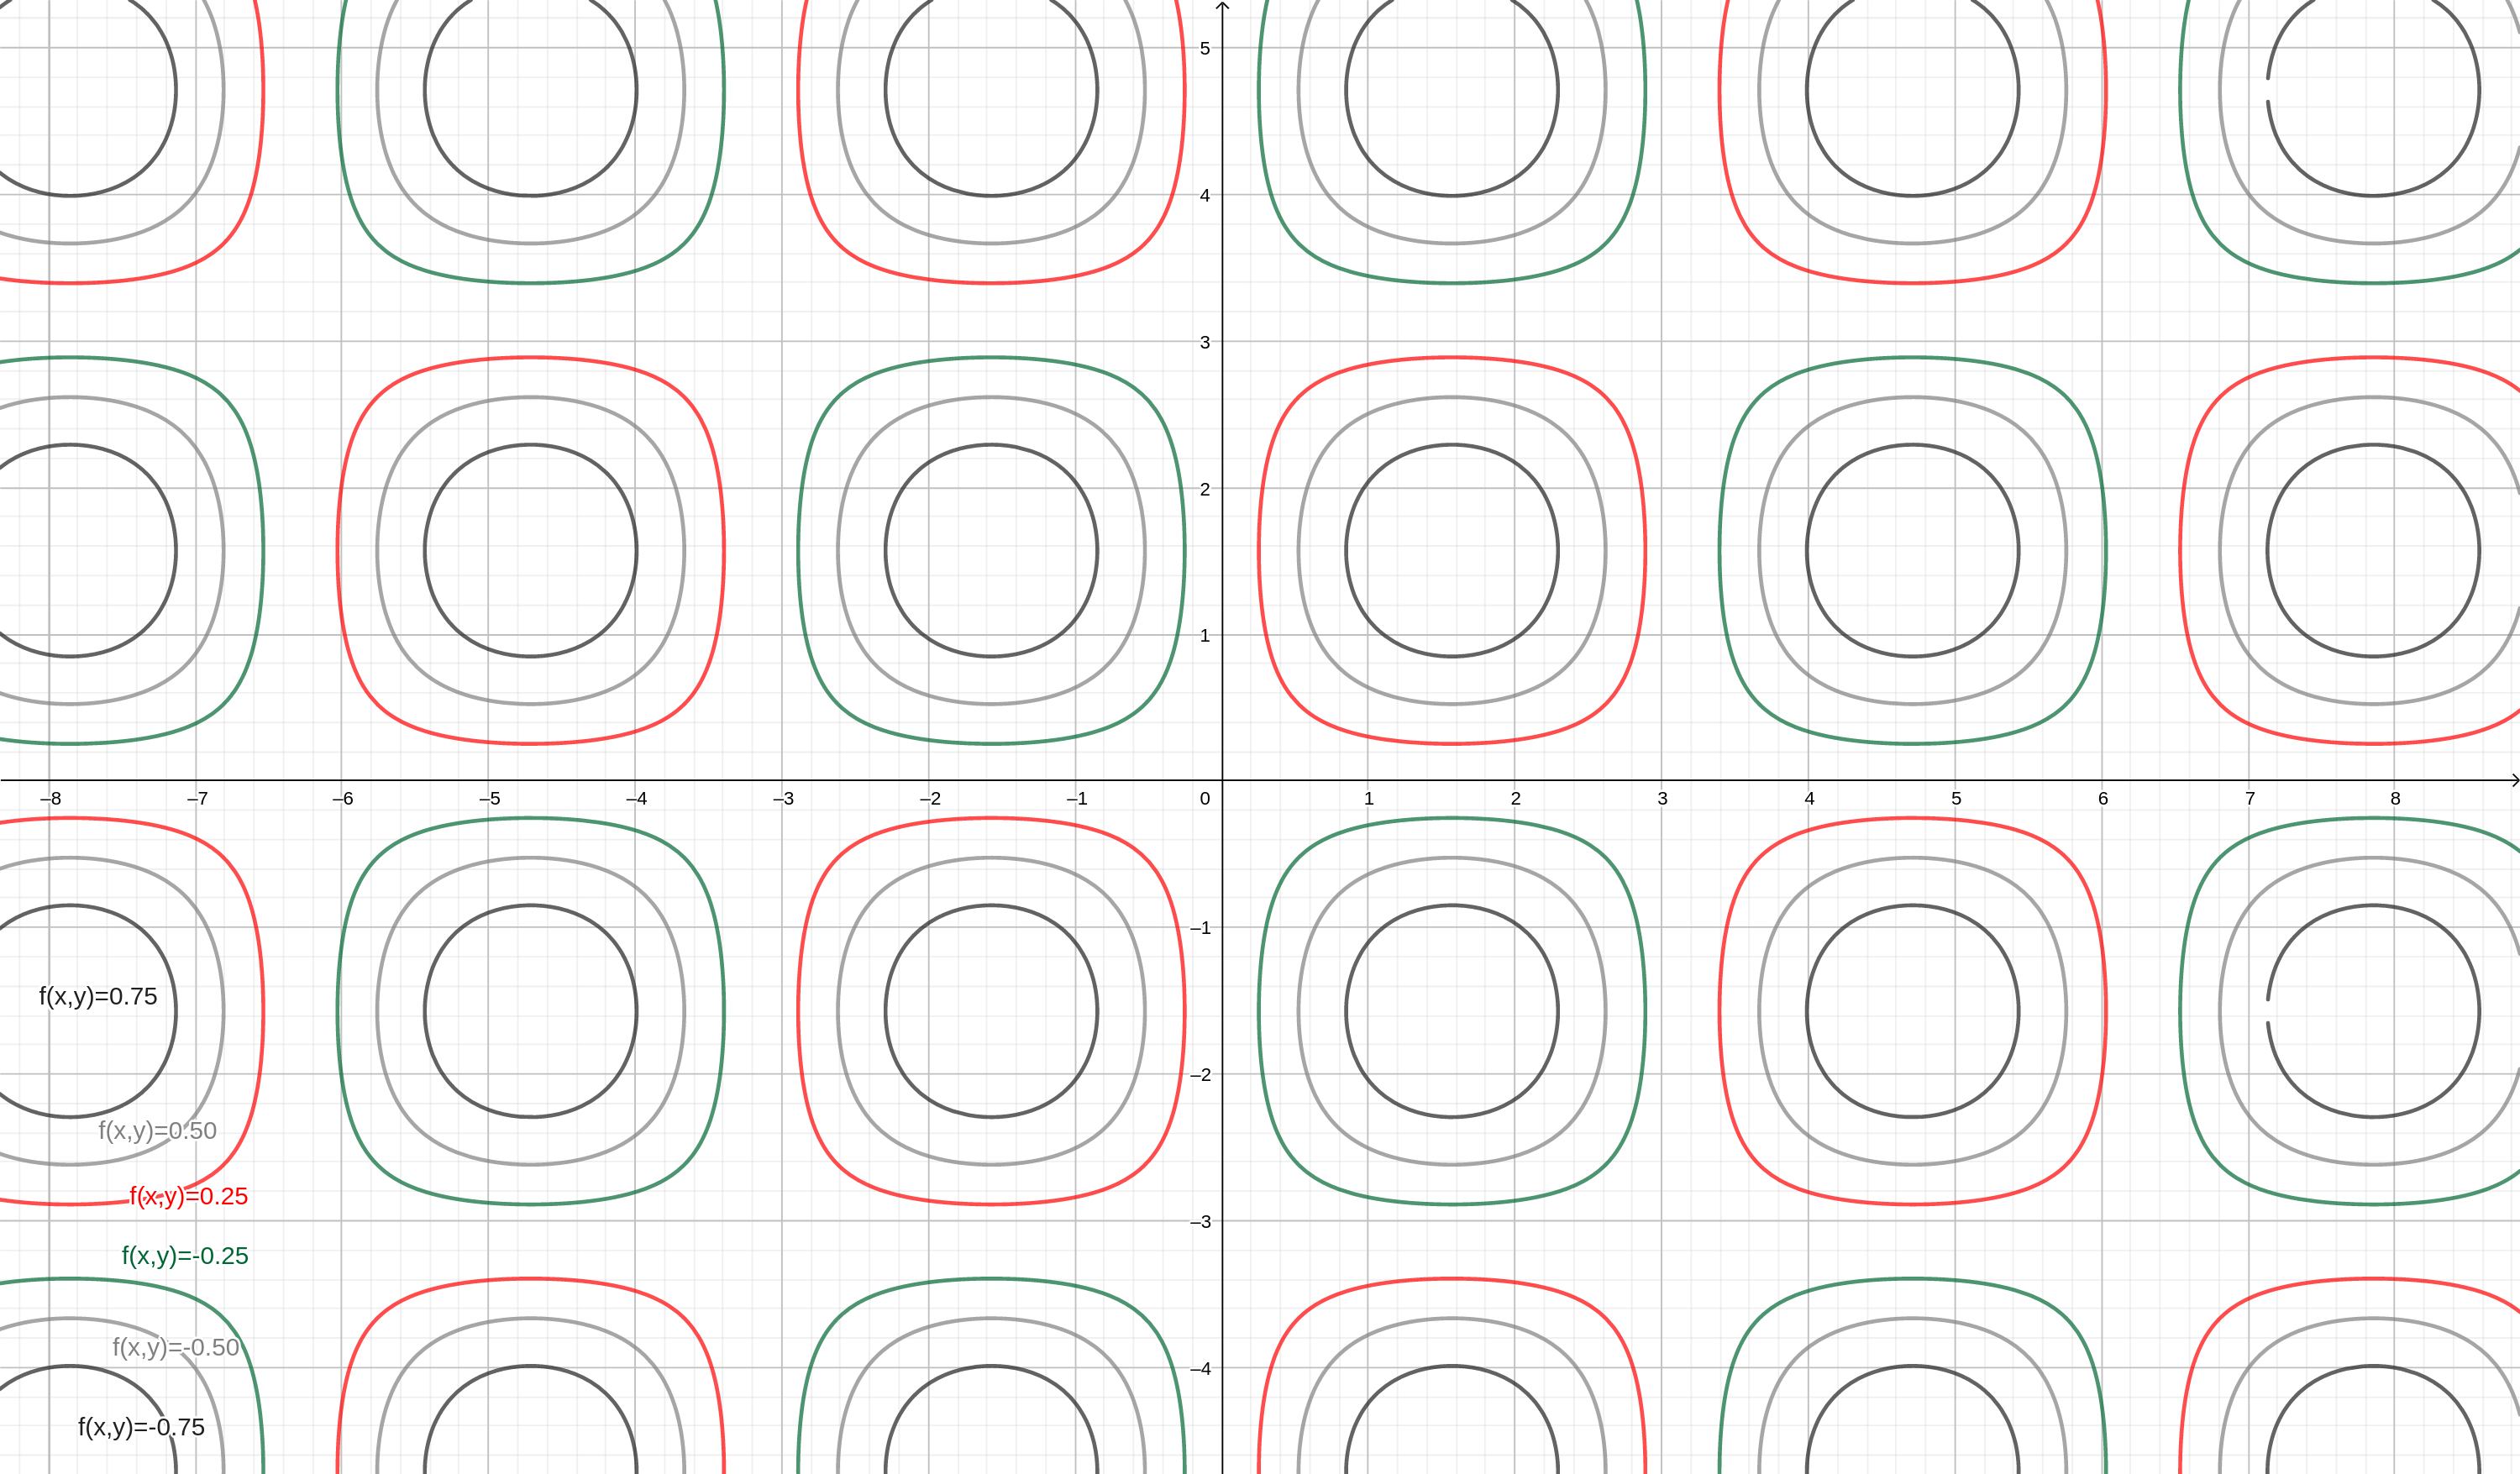
\includegraphics[width=0.9\textwidth]{../tex-snippets/ex-graph-contour-2-img-a.png}
  \caption{Ausgewählte Höhenlinien von $f(x,y)=\sin(x)\sin(y)$}
  \label{ex-graph-contour-2-img-a}
\end{figure}

\begin{figure}[ht]
  \centering
  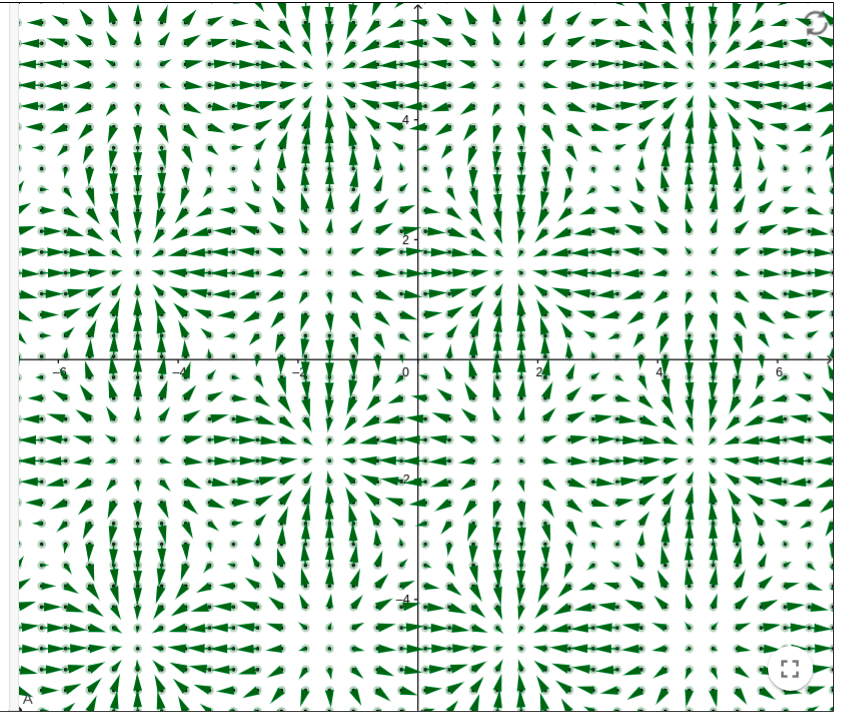
\includegraphics[width=0.9\textwidth]{../tex-snippets/ex-graph-contour-2-img-b.png}
  \caption{Gradientenfeld von $f(x,y)=\sin(x)\sin(y)$}
  \label{ex-graph-contour-2-img-b}
\end{figure}

\begin{figure}[ht]
  \centering
  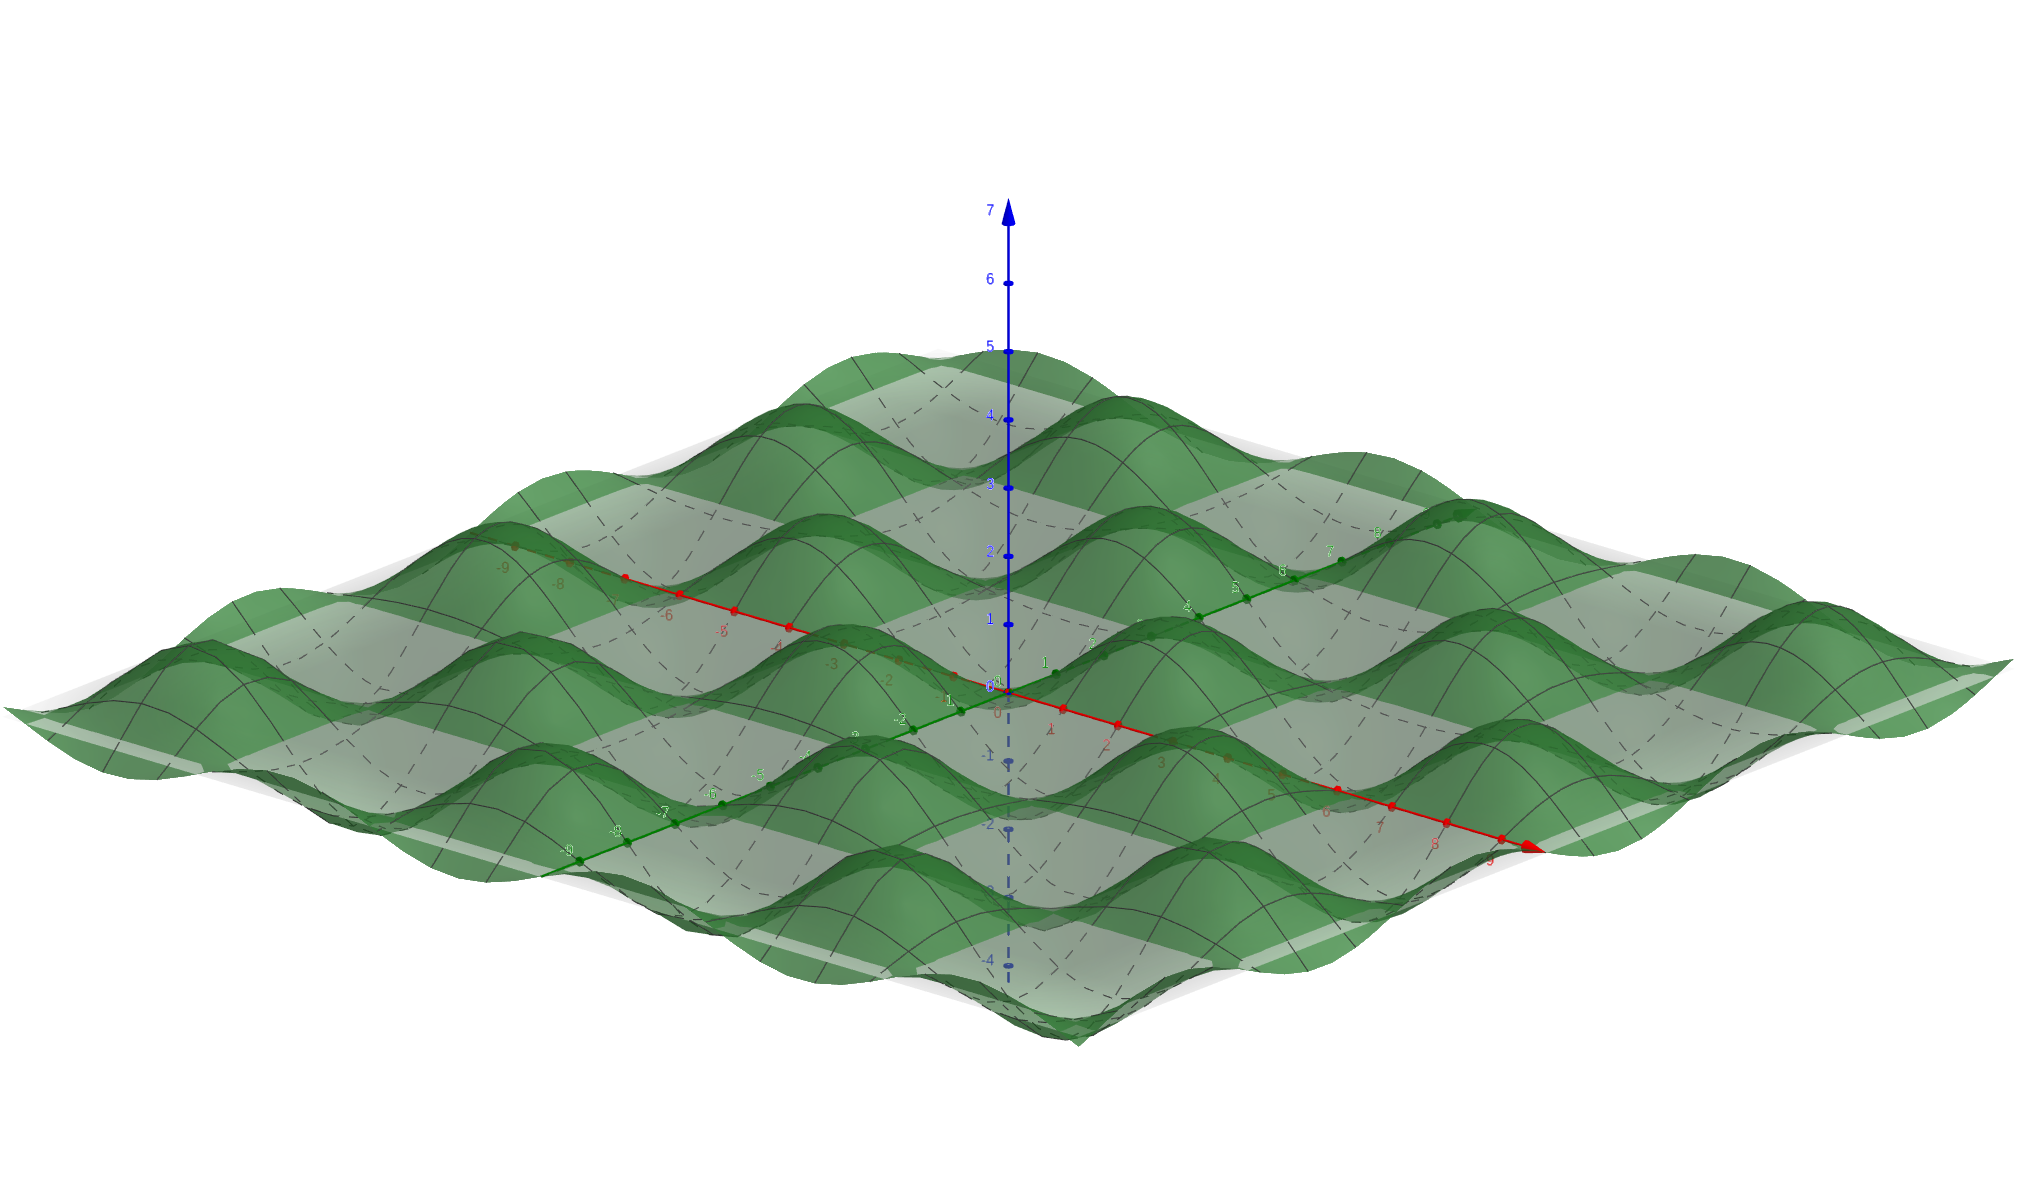
\includegraphics[width=0.9\textwidth]{../tex-snippets/ex-graph-contour-2-img-c.png}
  \caption{3D-Plot von $f(x,y)=\sin(x)\sin(y)$}
  \label{ex-graph-contour-2-img-c}
\end{figure}

